\icode{N17-MD-CA-L3-261112-002}
\nceeID[unkown]{2017全国\Rmnum{3}}{unkown}
如图，两个滑块 \(A\) 和 \(B\) 的质量分别为 \(m_1 =\) \,\qty{1}{kg}和 \(m_2 =\) \,\qty{5}{kg}，放在静止于水平地面上的木板的两端，两者与木板间的动摩擦因数均为 \(\mu_1 = 0.5\)；木板的质量为 \(m =\) \,\qty{4}{kg}，与地面间的动摩擦因数为 \(\mu_2 = 0.1\)。某时刻 \(A\)、\(B\) 两滑块开始相向滑动，初速度大小均为 \(v_0 =\) \,\qty{3}{m/s}。\(A\)、\(B\) 相遇时，\(A\) 与木板恰好相对静止。设最大静摩擦力等于滑动摩擦力，取重力加速度大小 \(g =\) \,\qty{10}{m/s^2}。求：
\begin{enumerate}
	\item \(B\) 与木板相对静止时，木板的速度；
	\item \(A\)、\(B\) 开始运动时，两者之间的距离。
\end{enumerate}

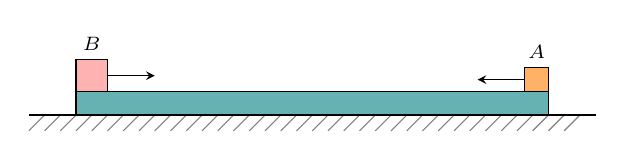
\begin{tikzpicture}[>=stealth,font=\scriptsize]
	\draw[fill=teal!60]	(0,0) rectangle(6,.3);
	\draw[fill=red!30] (0,.3) rectangle(.4,.7);
	\draw[->] (.4,.5)--++(.6,0);
	\node at(.2,.7)[above]{\(B\)};
	\draw[fill=orange!60] (5.7,.3) rectangle(6,.6);
	\draw[->] (5.7,.45)--++(-.6,0);
	\node at(5.85,.6)[above]{\(A\)};
	\foreach \x in {-.6,-.4,...,6.4}
		\draw[gray] (\x,-.2)--++(.2,.2);
	\draw[thick] (-.6,0)--(6.6,0);
\end{tikzpicture}
\begin{answer}
	（1）\qty{1}{m/s}（2）\qty{1.9}{m}
\end{answer}